\documentclass[svgnames,11pt]{beamer}
\input{/home/tof/Documents/Cozy/latex-include/preambule_commun.tex}
\input{/home/tof/Documents/Cozy/latex-include/preambule_beamer.tex}
%\usepackage{pgfpages} \setbeameroption{show notes on second screen=left}
\author[]{Christophe Viroulaud}
\title{Recherche de fichiers\\Notion d'arbre}
\date{\framebox{\textbf{Algo 04}}}
%\logo{}
\institute{Terminale - NSI}

\begin{document}
\begin{frame}
    \titlepage
\end{frame}
\begin{frame}[fragile]
    \frametitle{}

    Pour retrouver un document les systèmes d'exploitation proposent une fonction de recherche.
    \begin{center}
        \begin{lstlisting}[language=bash , basicstyle=\ttfamily\small, xleftmargin=2em, xrightmargin=2em]
find -name "mon-fichier.pdf"   
\end{lstlisting}
        \captionof{code}{\centering Rechercher \emph{mon-fichier.pdf} dans le dossier courant et ses sous-dossiers}
        \label{CODE}
    \end{center}

\end{frame}
\begin{frame}
    \frametitle{}

    \begin{framed}
        Comment effectuer une recherche efficace dans la structure des dossiers?
    \end{framed}

\end{frame}
\section{Structure hiérarchique arborescente}
\begin{frame}
    \frametitle{}


    \begin{center}
        \centering
        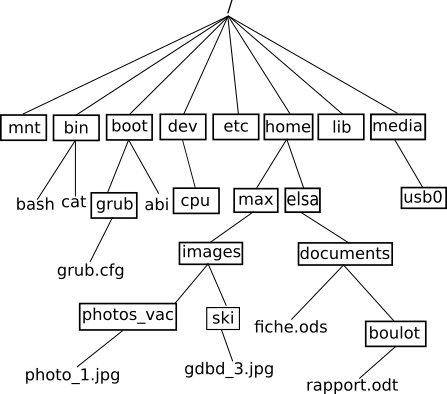
\includegraphics[width=8.5cm]{ressources/arbre-linux.png}
        \captionof{figure}{Structure hiérarchique d'un système Linux}
    \end{center}
\end{frame}
\begin{frame}
    \frametitle{}

    \begin{aretenir}[]
        Un arbre est défini par:
        \begin{itemize}
            \item un nœud particulier qui constitue la \textbf{racine},
            \item plusieurs sous-ensembles d'autres arborescences reliées à la racine.
        \end{itemize}
        On nomme \textbf{nœud-fils} l'ensemble des nœuds reliés à un même \textbf{nœud-père}.\\
        On nomme \textbf{feuilles} les nœuds qui n'ont pas de fils.
    \end{aretenir}

\end{frame}
\begin{frame}
    \frametitle{}

    \begin{aretenir}[Remarque]
        De manière usuelle un arbre est représentée \emph{à l'envers}, la racine en haut.
    \end{aretenir}
    \begin{center}
        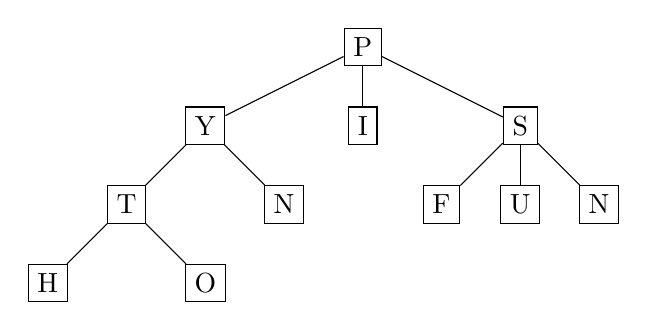
\begin{tikzpicture}
            \node[draw] (P) at (0,0) {P};
            \node[draw] (Y) at (-2,-1) {Y};
            \node[draw] (T) at (-3,-2) {T};
            \node[draw] (N) at (-1,-2) {N};
            \node[draw] (H) at (-4,-3) {H};
            \node[draw] (O) at (-2,-3) {O};
            \node[draw] (I) at (0,-1) {I};
            \node[draw] (S) at (2,-1) {S};
            \node[draw] (F) at (1,-2) {F};
            \node[draw] (U) at (2,-2) {U};
            \node[draw] (N2) at (3,-2) {N};
            \draw (P) -- (Y);
            \draw (T) -- (Y);
            \draw (T) -- (H);
            \draw (T) -- (O);
            \draw (N) -- (Y);
            \draw (P) -- (I);
            \draw (P) -- (S);
            \draw (F) -- (S);
            \draw (S) -- (U);
            \draw (N2) -- (S);
        \end{tikzpicture}
        \captionof{figure}{Une structure arborescente}
        \label{arbre}
    \end{center}
\end{frame}
\begin{frame}
    \frametitle{}

    \begin{aretenir}[]
        La \textbf{taille} d'un arbre est le nombre de nœuds de la structure.
    \end{aretenir}
    \begin{center}
        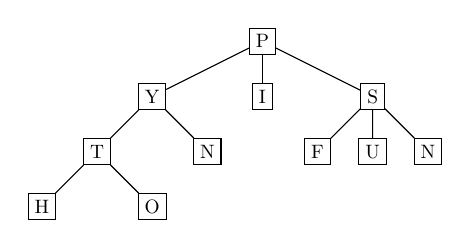
\begin{tikzpicture}[scale=0.7,transform shape]
            \node[draw] (P) at (0,0) {P};
            \node[draw] (Y) at (-2,-1) {Y};
            \node[draw] (T) at (-3,-2) {T};
            \node[draw] (N) at (-1,-2) {N};
            \node[draw] (H) at (-4,-3) {H};
            \node[draw] (O) at (-2,-3) {O};
            \node[draw] (I) at (0,-1) {I};
            \node[draw] (S) at (2,-1) {S};
            \node[draw] (F) at (1,-2) {F};
            \node[draw] (U) at (2,-2) {U};
            \node[draw] (N2) at (3,-2) {N};
            \draw (P) -- (Y);
            \draw (T) -- (Y);
            \draw (T) -- (H);
            \draw (T) -- (O);
            \draw (N) -- (Y);
            \draw (P) -- (I);
            \draw (P) -- (S);
            \draw (F) -- (S);
            \draw (S) -- (U);
            \draw (N2) -- (S);
        \end{tikzpicture}
        \captionof{figure}{La taille de l'arbre est 11.}
        \label{arbre}
    \end{center}
\end{frame}
\begin{frame}
    \frametitle{}

    \begin{aretenir}[]
        La \textbf{hauteur (ou profondeur)} d'un arbre est la longueur du plus grand chemin entre la racine et une feuille.
    \end{aretenir}
    \begin{center}
        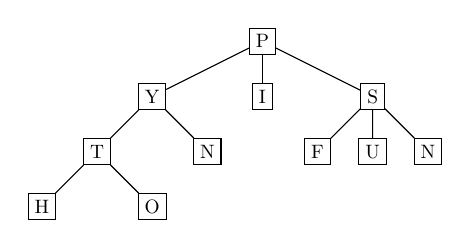
\begin{tikzpicture}[scale=0.7,transform shape]
            \node[draw] (P) at (0,0) {P};
            \node[draw] (Y) at (-2,-1) {Y};
            \node[draw] (T) at (-3,-2) {T};
            \node[draw] (N) at (-1,-2) {N};
            \node[draw] (H) at (-4,-3) {H};
            \node[draw] (O) at (-2,-3) {O};
            \node[draw] (I) at (0,-1) {I};
            \node[draw] (S) at (2,-1) {S};
            \node[draw] (F) at (1,-2) {F};
            \node[draw] (U) at (2,-2) {U};
            \node[draw] (N2) at (3,-2) {N};
            \draw (P) -- (Y);
            \draw (T) -- (Y);
            \draw (T) -- (H);
            \draw (T) -- (O);
            \draw (N) -- (Y);
            \draw (P) -- (I);
            \draw (P) -- (S);
            \draw (F) -- (S);
            \draw (S) -- (U);
            \draw (N2) -- (S);
        \end{tikzpicture}
        \captionof{figure}{La hauteur de l'arbre est 3.}
        \label{arbre}
    \end{center}
\end{frame}
\begin{frame}
    \frametitle{}

    \begin{aretenir}[Remarque]
        La définition de la \emph{hauteur} varie dans la littérature. Elle peut être présentée comme le nombre maximum de sommets entre la racine et une feuille. \emph{La hauteur de l'arbre est alors 4.}
    \end{aretenir}

\end{frame}
\section{Parcourir un arbre}
\subsection{Parcours en largeur}
\begin{frame}
    \frametitle{Parcours en largeur}

    \begin{aretenir}[]
        L'arbre est parcouru niveau par niveau. À chaque étage les nœuds sont parcourus avant de passer au niveau suivant. L'ordre des nœuds par niveau n'est pas déterminé.
    \end{aretenir}

\end{frame}
\begin{frame}
    \frametitle{}

    \begin{activite}
        Parcourir en largeur l'arbre suivant.
    \end{activite}
    \begin{center}
        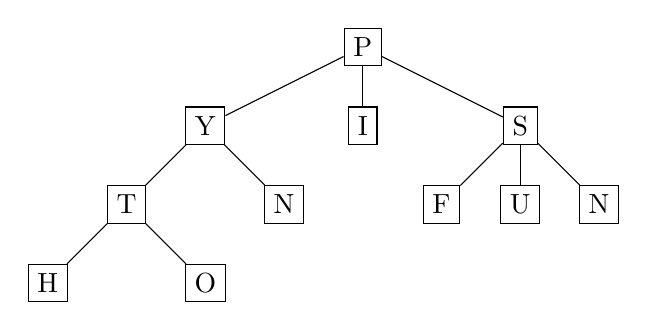
\begin{tikzpicture}
            \node[draw] (P) at (0,0) {P};
            \node[draw] (Y) at (-2,-1) {Y};
            \node[draw] (T) at (-3,-2) {T};
            \node[draw] (N) at (-1,-2) {N};
            \node[draw] (H) at (-4,-3) {H};
            \node[draw] (O) at (-2,-3) {O};
            \node[draw] (I) at (0,-1) {I};
            \node[draw] (S) at (2,-1) {S};
            \node[draw] (F) at (1,-2) {F};
            \node[draw] (U) at (2,-2) {U};
            \node[draw] (N2) at (3,-2) {N};
            \draw (P) -- (Y);
            \draw (T) -- (Y);
            \draw (T) -- (H);
            \draw (T) -- (O);
            \draw (N) -- (Y);
            \draw (P) -- (I);
            \draw (P) -- (S);
            \draw (F) -- (S);
            \draw (S) -- (U);
            \draw (N2) -- (S);
        \end{tikzpicture}
    \end{center}
\end{frame}
\begin{frame}
    \frametitle{Correction}
    \begin{center}
        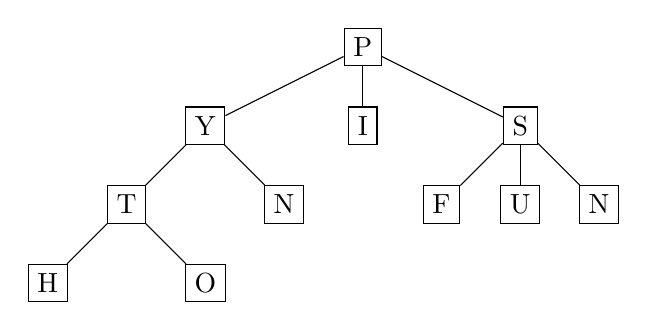
\begin{tikzpicture}
            \node[draw] (P) at (0,0) {P};
            \node[draw] (Y) at (-2,-1) {Y};
            \node[draw] (T) at (-3,-2) {T};
            \node[draw] (N) at (-1,-2) {N};
            \node[draw] (H) at (-4,-3) {H};
            \node[draw] (O) at (-2,-3) {O};
            \node[draw] (I) at (0,-1) {I};
            \node[draw] (S) at (2,-1) {S};
            \node[draw] (F) at (1,-2) {F};
            \node[draw] (U) at (2,-2) {U};
            \node[draw] (N2) at (3,-2) {N};
            \draw (P) -- (Y);
            \draw (T) -- (Y);
            \draw (T) -- (H);
            \draw (T) -- (O);
            \draw (N) -- (Y);
            \draw (P) -- (I);
            \draw (P) -- (S);
            \draw (F) -- (S);
            \draw (S) -- (U);
            \draw (N2) -- (S);
        \end{tikzpicture}
    \end{center}
    Parcours en largeur: P - Y - I - S - T - N - F - U - N - H - O

\end{frame}
\subsection{Parcours en profondeur}
\begin{frame}
    \frametitle{Parcours en profondeur}

    \begin{aretenir}[]
        Dans un parcours en profondeur, un des sous-arbres est parcouru entièrement avant qu'un autre ne soit exploré. C'est un algorithme récursif.
    \end{aretenir}
\end{frame}
\begin{frame}

    \begin{aretenir}[]On distingue trois parcours en profondeur:
        \begin{itemize}
            \item \textbf{ordre préfixe:} On liste \textbf{R} puis les nœuds de \textbf{$F_1$} en ordre préfixe, puis les nœuds de \textbf{$F_2$} en ordre préfixe\dots
            \item \textbf{ordre infixe:} On liste les nœuds de \textbf{$F_1$} en ordre infixe, puis \textbf{R}, puis les nœuds de \textbf{$F_2$} en ordre infixe\dots
            \item \textbf{ordre suffixe:} On liste les nœuds de \textbf{$F_1$} en ordre suffixe, puis les nœuds de \textbf{$F_2$} en ordre suffixe\dots, puis \textbf{R}.
        \end{itemize}
    \end{aretenir}
    \begin{center}

        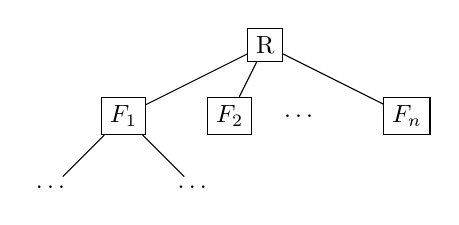
\begin{tikzpicture}[scale=.9, transform shape]
            \node[draw] (P) at (0,0) {R};
            \node[draw] (Y) at (-2,-1) {$F_1$};
            \node[draw] (I) at (-.5,-1) {$F_2$};
            \node (A) at (.5,-1) {\dots};
            \node[draw] (S) at (2,-1) {$F_n$};
            \node (B) at (-3,-2) {\dots};
            \node (C) at (-1,-2) {\dots};

            \draw (P) -- (Y);
            \draw (P) -- (I);
            \draw (P) -- (S);
            \draw (Y) -- (B);
            \draw (Y) -- (C);

        \end{tikzpicture}
    \end{center}
\end{frame}
\begin{frame}
    \frametitle{}

    \begin{activite}
        Parcourir en profondeur l'arbre suivant.
    \end{activite}
    \begin{center}
        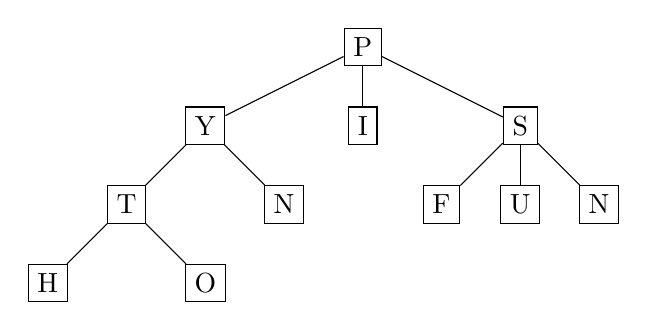
\begin{tikzpicture}
            \node[draw] (P) at (0,0) {P};
            \node[draw] (Y) at (-2,-1) {Y};
            \node[draw] (T) at (-3,-2) {T};
            \node[draw] (N) at (-1,-2) {N};
            \node[draw] (H) at (-4,-3) {H};
            \node[draw] (O) at (-2,-3) {O};
            \node[draw] (I) at (0,-1) {I};
            \node[draw] (S) at (2,-1) {S};
            \node[draw] (F) at (1,-2) {F};
            \node[draw] (U) at (2,-2) {U};
            \node[draw] (N2) at (3,-2) {N};
            \draw (P) -- (Y);
            \draw (T) -- (Y);
            \draw (T) -- (H);
            \draw (T) -- (O);
            \draw (N) -- (Y);
            \draw (P) -- (I);
            \draw (P) -- (S);
            \draw (F) -- (S);
            \draw (S) -- (U);
            \draw (N2) -- (S);
        \end{tikzpicture}
    \end{center}
\end{frame}
\begin{frame}
    \frametitle{Correction}
    \begin{center}
        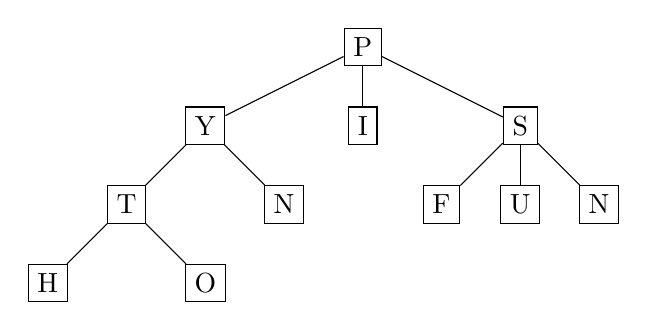
\begin{tikzpicture}
            \node[draw] (P) at (0,0) {P};
            \node[draw] (Y) at (-2,-1) {Y};
            \node[draw] (T) at (-3,-2) {T};
            \node[draw] (N) at (-1,-2) {N};
            \node[draw] (H) at (-4,-3) {H};
            \node[draw] (O) at (-2,-3) {O};
            \node[draw] (I) at (0,-1) {I};
            \node[draw] (S) at (2,-1) {S};
            \node[draw] (F) at (1,-2) {F};
            \node[draw] (U) at (2,-2) {U};
            \node[draw] (N2) at (3,-2) {N};
            \draw (P) -- (Y);
            \draw (T) -- (Y);
            \draw (T) -- (H);
            \draw (T) -- (O);
            \draw (N) -- (Y);
            \draw (P) -- (I);
            \draw (P) -- (S);
            \draw (F) -- (S);
            \draw (S) -- (U);
            \draw (N2) -- (S);
        \end{tikzpicture}
    \end{center}
    \begin{itemize}
        \item Parcours préfixe: P - Y - T - H - O - N - I - S - F - U - N
        \item Parcours infixe: H - T - O - Y - N - P - I - F - S - U - N
        \item Parcours suffixe: H - O - T - N - Y - I - F - U - N - S - P
    \end{itemize}

\end{frame}
\subsection{Rechercher un fichier}
\begin{frame}[fragile]
    \frametitle{Rechercher un fichier}
        \begin{center}
            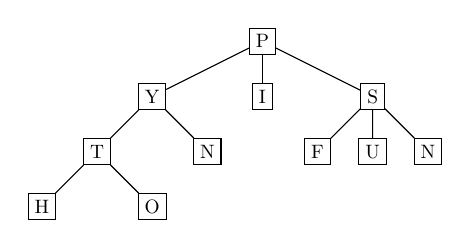
\begin{tikzpicture}[scale=.7, transform shape]
                \node[draw] (P) at (0,0) {P};
                \node[draw] (Y) at (-2,-1) {Y};
                \node[draw] (T) at (-3,-2) {T};
                \node[draw] (N) at (-1,-2) {N};
                \node[draw] (H) at (-4,-3) {H};
                \node[draw] (O) at (-2,-3) {O};
                \node[draw] (I) at (0,-1) {I};
                \node[draw] (S) at (2,-1) {S};
                \node[draw] (F) at (1,-2) {F};
                \node[draw] (U) at (2,-2) {U};
                \node[draw] (N2) at (3,-2) {N};
                \draw (P) -- (Y);
                \draw (T) -- (Y);
                \draw (T) -- (H);
                \draw (T) -- (O);
                \draw (N) -- (Y);
                \draw (P) -- (I);
                \draw (P) -- (S);
                \draw (F) -- (S);
                \draw (S) -- (U);
                \draw (N2) -- (S);
            \end{tikzpicture}
        \end{center}
    \begin{activite}
        \begin{enumerate}
            \item Ouvrir l'ordinateur virtuel sous Debian.
            \item Créer l'arborescence de dossiers représentée par l'arbre, à l'aide des instructions suivantes:\\
            \begin{lstlisting}[language=bash , basicstyle=\ttfamily\small, xleftmargin=2em, xrightmargin=0em]
mkdir p # Créer le dossier p
cd p # Entrer dans le dossier p
cd .. # Retourner dans le dossier père
\end{lstlisting}
        \end{enumerate}
    \end{activite}

\end{frame}
\begin{frame}[fragile]
    \frametitle{}

    \begin{activite}
    \begin{enumerate}
        \setcounter{enumi}{2}
        \item Se placer dans le dossier \textbf{P}.
            \item La commande suivante affiche le parcours d'une recherche quelconque. L'exécuter.
            \begin{lstlisting}[language=bash , basicstyle=\ttfamily\small, xleftmargin=2em, xrightmargin=2em]
find -print
\end{lstlisting}
            \item Quel type de parcours effectue la fonction \emph{find}?
    \end{enumerate}
    \end{activite}

\end{frame}
\begin{frame}[fragile]
    \frametitle{Correction}

    \begin{center}
    \begin{lstlisting}[language=Python , basicstyle=\ttfamily\small, xleftmargin=2em, xrightmargin=2em]
.
./y
./y/t
./y/t/h
./y/t/o
./y/n
./y/n/i
./s
./s/f
./s/u
./s/u/n
\end{lstlisting}
    \captionof{code}{Parcours en profondeur préfixe}
    \label{CODE}
    \end{center}

\end{frame}
\end{document}